\chapter{Conceção}
\label{chap:Chapter4}
Neste capítulo apresenta-se o processo de idealização do módulo de linguagem natural. Inicialmente, explica-se o processo de experimentação de algumas ferramentas ou abordagens analisadas no capítulo anterior, procurando perceber se a sua aplicação prática é plausível. Depois, mostra-se o modelo concetualizado, concretamente a visão geral, em que se faz uma descrição do modelo na sua globalidade, os casos de uso identificados e por fim, a arquitetura definida.

%%%%%%%%%%%%%%%%%%%%%%%%%%%%%%%%%
%           SECTION
%%%%%%%%%%%%%%%%%%%%%%%%%%%%%%%%%
\section{Apreciação Prática}
\label{sec:chap04_approaches}
Com o propósito de colocar em prática o estudo das \glspl{iln}, decidiu-se a realização de experiências envolvendo algumas abordagens e ferramentas previamente estudadas (ver Capítulo~\ref{chap:Chapter3}). Posto isto, optou-se por desenvolver pequenas provas de conceito, de forma a fazer uma rápida avaliação das abordagens, técnicas e ferramentas usadas. Para cada uma, é abordado em que consiste, algumas observações pertinentes e referência dos pontos favoráveis e desfavoráveis.

\subsection{Gramática Baseada em Semântica}
Como proposto em~\textcite[p.~361-403]{natural_language_processing_with_python}, o uso do NLTK permite o desenvolvimento de gramáticas que possibilitam a análise de uma frase pela sua semântica, tal como o exemplo demonstrado a seguir.

\begin{lstlisting}[language={},caption={Excerto de uma gramática, extraído de~\textcite{natural_language_processing_with_python}},numbers=none,label=lst:grammarexample,basicstyle=\scriptsize]
S[SEM=(?np + WHERE + ?vp)] -> NP[SEM=?np] VP[SEM=?vp]
VP[SEM=(?v + ?pp)] -> IV[SEM=?v] PP[SEM=?pp]
VP[SEM=(?v + ?ap)] -> IV[SEM=?v] AP[SEM=?ap]
NP[SEM=(?det + ?n)] -> Det[SEM=?det] N[SEM=?n]
PP[SEM=(?p + ?np)] -> P[SEM=?p] NP[SEM=?np]
AP[SEM=?pp] -> A[SEM=?a] PP[SEM=?pp]
NP[SEM='Country="greece"'] -> 'Greece'
NP[SEM='Country="china"'] -> 'China'
Det[SEM='SELECT'] -> 'Which' | 'What'
N[SEM='City FROM city_table'] -> 'cities'
IV[SEM=''] -> 'are'
A[SEM=''] -> 'located'
P[SEM=''] -> 'in'
\end{lstlisting}

O código apresentado em~\ref{lst:grammarexample}, usando o NLTK, para a pergunta \inquotes{What cities are located in China?} permite gerar a seguinte \textit{query} de \gls{sql}: \textit{SELECT City FROM city\_table WHERE Country=\inquotes{china}}. Com esta metodologia é possível mapear diretamente linguagem natural em \gls{sql}, sendo que a gramática funciona como a base de conhecimento. Por conseguinte, torna-se viável a codificação de um \textit{parser} que usa as gramáticas definidas, verificando
alguma é capaz de dar resposta à \textit{query} de linguagem natural.

\subsubsection*{Pontos Favoráveis}
\begin{itemize}
    \item 
    {
        Viabilidade de desenvolvimento de uma solução customizada;
    }
    \item
    {
        Utilização de ferramenta \textit{open source};
    }
    \item 
    {
        Tradução imediata de linguagem natural para \gls{sql}. 
    }
\end{itemize}

\subsubsection*{Pontos Desfavoráveis}
\begin{itemize}
    \item 
    {
        Dificuldade em criar ou estender gramáticas;
    }
    \item
    {
        Complexidade em adaptar para múltiplas línguas ou domínios;
    }
    \item
    {
        Necessidade de conhecimento linguístico, por forma a adaptar a gramática às regras de uma determinada língua;
    }
    \item
    {
        Ambiguidade da semântica. Diferentes expressões podem ou devem gerar o mesmo \gls{sql};
    }
    \item
    {
        Manutenção difícil.
    }
\end{itemize}

\subsection{Pesquisa Semântica}
Nesta abordagem usou-se uma \textit{framework} que não consta nas ferramentas estudadas (ver Secção~\ref{sec:chap03_existingtools}), principalmente porque o seu desenvolvimento encontra-se estagnado desde 2013. Ainda assim, contemplou-se o seu uso para testar esta abordagem, no ponto de vista prático. O Quepy foi desenvolvido em \textit{Python} e tem como objetivo a transformação de linguagem natural em \textit{SPARQL Protocol and RDF Query Language} (SPARQL)\footnote{Disponível em \url{https://www.w3.org/TR/rdf-sparql-query/}.} e \textit{Metaweb Query Language} (MQL)\footnote{Disponível em \url{https://github.com/nchah/freebase-mql}.}, linguagens de \textit{query} usadas com tecnologia \gls{rdf}\footnote{Disponível em \url{https://www.w3.org/RDF/}.}, \inquotes{um modelo padrão para permuta de dados na Web}\footnote{Tradução livre do autor. No original \inquotes{is a standard model for data interchange on the Web.}.}, intrinsecamente ligado ao campo da Web Semântica~\parencite{resource_description_framework}.

Neste caso, o uso do Quepy implicou a definição da linguagem específica de domínio através de código \textit{Python}, respeitando as restrições colocadas na documentação da \textit{framework}, de maneira a que esta fosse capaz de reconhecer o padrão introduzido.

\begin{lstlisting}[language=python, caption={Excerto da definição semântica da frase que lida com listagem de produtos},numbers=none,label=lst:quepyexample,basicstyle=\scriptsize]
from quepy.dsl import FixedType, FixedRelation
from quepy.parsing import Lemma, QuestionTemplate

class NameOf(FixedRelation):
    "Name of the entity's property"
    relation = "product_name"
    reverse = True

class IsProduct(FixedType):
    "Defines the entity's type"
    fixedtype = "product"

class ListProducts(QuestionTemplate):
    "Questions such as 'List products' or 'Listing products'"
    regex = Lemma("list") + Lemma("product")

    def interpret(self, match):
        product = IsProduct()
        name = NameOf(product)
        return name, "enum"

\end{lstlisting}

No excerto demonstrado em~\ref{lst:quepyexample}, define-se a expressão regular que caracteriza a questão esperada, para além de detalhes relacionados com a linguagem específica de domínio. A \textit{query} obtida pode ser posteriormente usada numa base de dados \gls{rdf}, como o objetivo de recolher os dados. De notar que, neste caso, sendo o propósito a consulta de uma base de dados relacional, seria necessária uma forma de a transpor ou replicar numa camada compatível com tecnologia \gls{rdf}. Para isso, existem ferramentas capazes de executar esse mapeamento, como por exemplo o D2RQ\footnote{Disponível em \url{http://d2rq.org/}.}.

\subsubsection*{Pontos Favoráveis}
\begin{itemize}
    \item
    {
        Viabilidade de desenvolvimento de uma solução customizada;
    }
    \item
    {
        Tecnologia \textit{open source};
    }
    \item 
    {
        Linguagem específica de domínio permite abstração aos detalhes de implementação associados ao reconhecimento de linguagem natural;
    }
    \item
    {
        Reconhecimento da linguagem natural é feita através da análise de expressões regulares, o que torna fácil compreender a estrutura frásica;
    }
    \item
    {
        Transformação da linguagem natural numa representação que obedece à especificação da tecnologia \gls{rdf}, definida pela W3C.
    }
\end{itemize}

\subsubsection*{Pontos Desfavoráveis}
\begin{itemize}
    \item
    {
        As regras de domínio e o modelo de dados devem ser definidos diretamente no código, não possibilitando a extensibilidade por configuração;
    }
    \item
    {
        Rigidez da linguagem usada, já que o uso de expressões regulares implica uma estrutura minimamente estática para que o reconhecimento seja bem sucedido;
    }
    \item
    {
        O uso de tecnologias \gls{rdf} levam a uma nova camada aplicacional, que envolve o uso de ferramentas não relacionadas com o \gls{pln} e que leva a mais esforço na manutenção do sistema;
    }
    \item
    {
        Necessidade de estudo aprofundado ou conhecimento pericial na área de Web Semântica.
    }
\end{itemize}

\subsection{Reconhecimento de Intenções e Entidades}
Neste contexto, utilizou-se o Microsoft LUIS, uma das ferramentas previamente estudadas (ver Secção~\ref{sec:chap03_existingtools}). A razão para esta escolha deve-se principalmente a dois fatores: o facto de ser uma plataforma bastante documentada e pela Microsoft disponibilizar (ainda que de forma limitada) este tipo de ferramentas a quem possua subscrição de estudante. 

Para esta prova de conceito criou-se um \textit{chatbot} capaz de responder a algumas perguntas colocadas pelo utilizador, identificando qual a sua intenção e quais as entidades envolvidas, como se apresenta a seguir:
%
\begin{itemize}
    \item
    {
        \textit{Good Morning} -- corresponde à intenção de \textit{Greeting} (saudação), não existindo entidades associadas;
    }
    \item
    {
        \textit{What's the weather like in \underline{Porto}?} -- intenção de \textit{CheckWeather} (verificar condições meteorológicas), cuja entidade dinâmica é o \textit{Place} (lugar) indicado pelo utilizador.
    }
    \item
    {
        \textit{Book me a flight to \underline{Lisbon} \underline{next week}} -- intenção de \textit{BookFlight} (agendar voo), que possui duas entidades dinâmicas: o lugar de destino (\textit{Place}) e o momento da viagem (\textit{Datetime}).
    }
\end{itemize}

% , descritas na Tabela~\ref{tab:luis_intents}.
% %
% \begin{table}
% \caption{Descrição de algumas das intenções e entidades dada a expressão de exemplo, baseado em~\textcite[Concepts]{microsoft_luis_official}}
% \label{tab:luis_intents}
% \centering
% \resizebox{\textwidth}{!}{
% \renewcommand{\arraystretch}{1.3}
% \footnotesize
% \begin{tabular}{l*{2}{|l}}
%
\toprule
%
\tabhead{Expressão de Exemplo}&\tabhead{Intenção}&\tabhead{Entidades}\\
%
\midrule
%
{Good Morning}&{Greeting}&{--}\\
%
{What's the weather like in \underline{Porto}?}&{CheckWeather}&{Place}\\
%
{Turn on the Internet in my \underline{bedroom}, please}&{HomeAutomation}&{Room}\\
%
{Book me a flight to \underline{Lisbon} \underline{next week}}&{BookFlight}&{Place, Datetime}\\
%
\bottomrule
%
\end{tabular}
% }
% \end{table}

O \textit{chatbot} recorreu ao Microsoft LUIS para a identificar a intenção do utilizador, e com base nisso, respondia com a intenção e entidades que foi capaz de identificar (ver Figura~\ref{fig:chatbotexample}). 
%
\begin{figure}
\centering
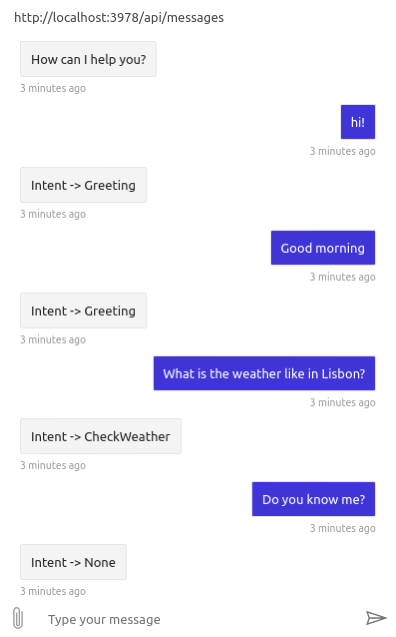
\includegraphics[width=.45\textwidth]{ch04/assets/chatbot.jpg}
\caption{Amostra de teste com \textit{chatbot} desenvolvido usando Microsoft LUIS}
\label{fig:chatbotexample}
\end{figure}
%
Notou-se ser possível dotar o \textit{chatbot} de comportamento para manipular os metadados obtidos, e assim, obter dados de uma base de dados relacional ou obter dados estáticos dum serviço de respostas pré-fabricadas, tal como o QnA Maker\footnote{Disponível em \url{https://www.qnamaker.ai/}}.

\subsubsection*{Pontos Favoráveis}
\begin{itemize}
    \item
    {
        As plataformas disponíveis na \textit{cloud} constituem um ponto de partida para uma solução personalizada;
    }
    \item
    {
        A solução é fácil de desenvolver, estender e integrar;
    }
    \item
    {
        A base de conhecimento pode ser totalmente configurável;
    }
    \item
    {
        Robustez na identificação de intenções e entidades, através do uso de modelos de \gls{ml};
    }
\end{itemize}

\subsubsection*{Pontos Desfavoráveis}
\begin{itemize}
    \item
    {
        A aplicação desta abordagem numa biblioteca customizada implica o estudo teórico de \gls{ml} aplicado ao \gls{pln} e consequentemente, maior esforço de desenvolvimento;
    }
    \item
    {
        A adição de novas intenções à base de conhecimento leva também à adição de comportamento para lidar com os mesmas.
    }
\end{itemize}

\subsection{Sinopse}
As abordagens descritas anteriormente baseiam-se nas observações e experiências realizadas, no ponto de vista prático. Portanto, a conclusão aqui exposta leva em consideração os pontos favoráveis e desfavoráveis de cada uma.

A abordagem que parece a mais adequada é a que diz respeito ao reconhecimento de intenções e entidades, principalmente pela facilidade de compreensão e aplicação do conceito. Além do mais, os pontos desfavoráveis mencionados são de índole operacional, pelo que não parecem comprometer a conceção de um modelo e desenvolvimento do respetivo protótipo. 

Relativamente às abordagens descartadas, aponta-se que a primeira -- gramática baseada em semântica -- se usada no contexto comercial, seria difícil manter o seu desenvolvimento e capacidade de cobrir uma gama aceitável de questões válidas. Já a segunda -- pesquisa semântica --, ainda que assente sobre uma tecnologia especificada e aprovada pelo W3C, necessitaria de uma camada adicional (\gls{rdf}), contribuindo assim para o aumento do esforço em configuração e manutenção do sistema. Por isso, a terceira abordagem revela-se a mais adequada e será contemplada no protótipo a desenvolver.

%%%%%%%%%%%%%%%%%%%%%%%%%%%%%%%%%
%           SECTION
%%%%%%%%%%%%%%%%%%%%%%%%%%%%%%%%%
\section{Modelo Proposto}
\label{sec:chap04_proposal}
O estudo das \glspl{iln}, associado à aplicação prática de algumas ferramentas e abordagens estudadas, permitiram retirar conclusões relevantes de considerar na conceção do módulo. Nesta secção apresenta-se o modelo idealizado segundo uma abordagem de reconhecimento de intenções e entidades.

\subsection{Visão Geral}
A visão incide na conceção um módulo de linguagem natural para interface com o {\productname}, que permita aos operadores de linha, engenheiros de produção e gestores, consultar informação acerca do processo fabril. Como se apresenta na Figura~\ref{fig:generic-vision}, o sistema \gls{mes} disponibiliza uma interface para que o utilizador interaja com ele, através de texto, esperando obter informação relevante do processo, no formato que melhor se enquadrar.
%
\begin{figure}[!ht]
    \centering
    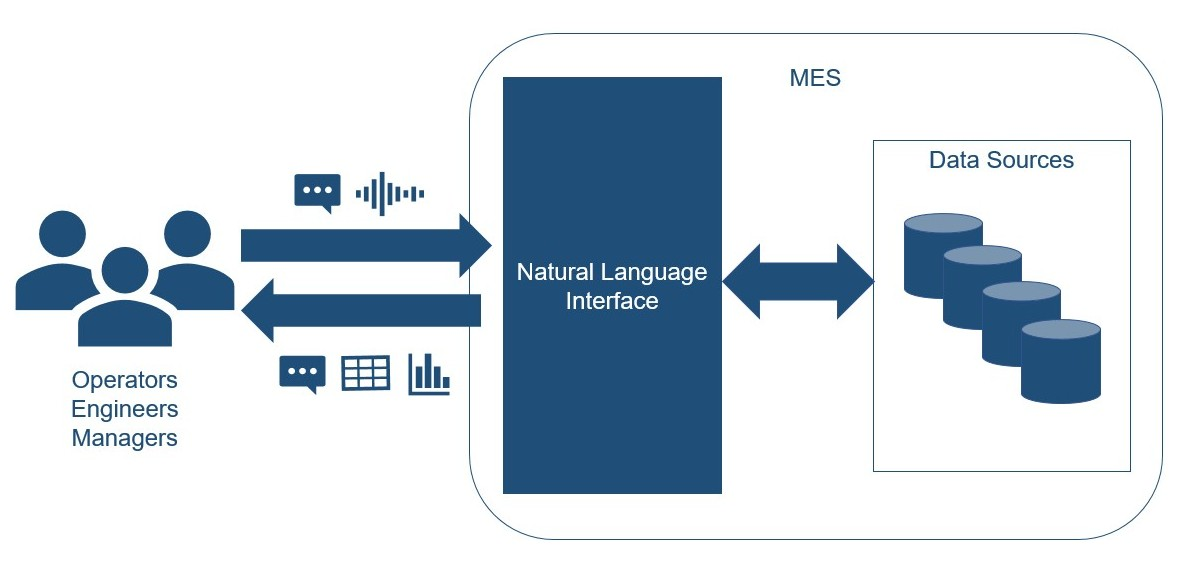
\includegraphics[width=.9\textwidth]{ch04/assets/generic-vision.jpg}
    \caption{Visão da solução desejada para o produto}
    \label{fig:generic-vision}
\end{figure}

O modelo tem em conta três fatores: a experiência de utilizador, a extensibilidade das bases de conhecimento e integração com o {\productname}. Relativamente à estratégia de reconhecimento de intenções e entidades a ser aplicada no modelo, definem-se os conceitos que lhe estão inerentes, apresentados na Figura~\ref{fig:domain_model}:

\begin{itemize}
    \item
    {
        \textit{Dynamic Knowledge Base} -- Base de conhecimento dinâmica. Fonte de dados que liga as expressões às intenções e entidades correspondentes e é usado no treino dos modelos \gls{ml} para previsão;
    }
    \item
    {
        \textit{Static Knowledge Base} -- Base de conhecimento estática. Dicionário onde consta uma determinada expressão e respetiva resposta. Pode ser usada para implementar conversação casual ou lidar com expressões que não constam na base de dados dinâmica;
    }
    \item
    {
        \textit{Intent} -- Intenção. Mapeia ação que o utilizador deseja executar. Normalmente estão-lhe associadas diversas expressões;
    }
    \item
    {
        \textit{Expression} -- Expressão. Corresponde ao exemplo de estrutura de uma pergunta que o utilizador pode fazer;
    }
    \item
    {
        \textit{Entity} -- Entidade. Tipicamente refere-se a um conceito de domínio ou do mundo real;
    }
    \item
    {
        \textit{Static Answer} -- Resposta Estática. Definida na base de conhecimento estática, associada a diferentes expressões. Por exemplo, expressões como \inquotes{Olá} ou \inquotes{Viva} podem ter associadas respostas como \inquotes{Oi} e \inquotes{Olá}.
    }
\end{itemize}
%
\begin{figure}
    \centering
    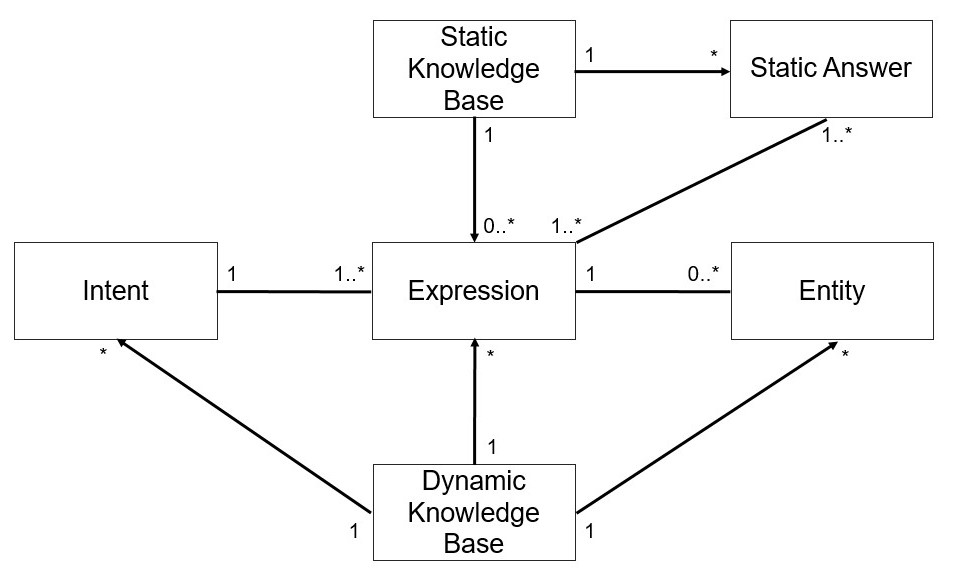
\includegraphics[width=.75\textwidth]{ch04/assets/domain-model.jpg}
    \caption{Conceitos associados ao reconhecimento de intenções e entidades e os respetivos relacionamentos}
    \label{fig:domain_model}
\end{figure}
%
Portanto, uma intenção é um conceito composto, base do modelo, que se apresenta como uma indireção face à questão colocada pelo utilizador, ou seja, a questão é analisada pela ação que lhe está associada e não propriamente pelo seu significado, \exempligratia{um pedido para obter os materiais mais fabricados num determinado setor constitui uma intenção única, apesar de apresentar entidades diferentes, consoante o domínio}.

\subsection{Casos de Uso}
De um ponto de vista de utilização, o modelo aqui proposto deve saber lidar com \textit{Perguntas}, \textit{Respostas} e \textit{Bases de Conhecimento}, que se podem considerar as principais áreas funcionais de sistema. Todas têm implicações no comportamento do módulo. Em relação às \textit{Perguntas} e \textit{Respostas}, uma vez que estão profundamente ligadas, apresentando funcionalidades comuns, são então enquadradas numa área funcional única, denominada \textit{QA}. A Figura~\ref{fig:use_cases} dá uma visão geral das áreas funcionais do sistema, que são descritas em seguida:
%
\begin{figure}
    \centering
    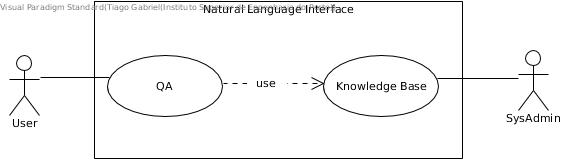
\includegraphics[width=.72\textwidth]{ch04/assets/use-cases.jpg}
    \caption{Áreas funcionais de sistema}
    \label{fig:use_cases}
\end{figure}
%
\begin{itemize}
    \item 
    {
        \textit{QA} -- corresponde ao conjunto de funcionalidades relacionadas com as perguntas colocadas pelos utilizadores e respetiva procura de respostas;
    }
    % \item 
    % {
    %     \textit{Feedback} -- conjunto de funções de sistema que lida com a recolha de \textit{feedback} do utilizador, para contribuir para a melhoria contínua da qualidade das respostas;
    % }
    \item 
    {
        \textit{Knowledge Base} -- área funcional \textit{Base de Conhecimento}. Apresenta funcionalidades para a gestão de intenções, expressões, entidades, ou seja, tudo o que as restantes áreas funcionais necessitam para o seu funcionamento.
    }
\end{itemize}

A área funcional \textit{QA} é essencial no contexto deste trabalho, já que se trata da base de interação com o utilizador. Por isso, a Figura~\ref{fig:detailed_use_cases}, apresentada a seguir, detalha algo mais essa área funcional.
%
\begin{figure}[!ht]
    \centering
    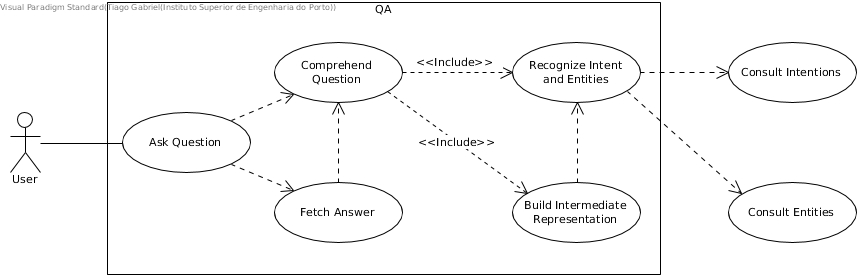
\includegraphics[width=.93\textwidth]{ch04/assets/questions-use-cases.jpg}
    \caption{Casos de uso identificados para a área funcional \textit{QA}}
    \label{fig:detailed_use_cases}
\end{figure}

Os casos de uso apresentados no diagrama são descritos a seguir:
\begin{itemize}
    \item 
    {
        \textit{Ask Question} -- Fazer Pergunta. É a funcionalidade principal. O utilizador faz a pergunta com o objetivo de obter a resposta que procura. Depende da compreensão da pergunta e da obtenção de resposta;
    }
    \item 
    {
        \textit{Comprehend Question} -- Compreender a Pergunta. O sistema procura compreender a pergunta feita e traduz para uma representação passível de ser usada na fase de procura da resposta nas fontes de dados disponíveis;
    }
    \item 
    {
        \textit{Recognize Intent and Entities} -- Reconhecer a Intenção e as Entidades. O sistema faz o reconhecimento da intenção e das entidades da pergunta feita com base no modelo de \gls{ml} treinado com os dados que constam na base de conhecimento;
    }
    \item 
    {
        \textit{Build Intermediate Representation} -- Construir Representação Intermédia. O sistema constrói uma representação intermediária que contém os metadados da pergunta colocada -- intenção, entidades e outros dados relevantes;
    }
    \item 
    {
        \textit{Consult Intentions} -- Consultar as Intenções. Permite a consulta de intenções mantidas na base de conhecimento;
    }
    \item 
    {
        \textit{Consult Entities} -- Consultar as Entidades. Permite a consulta as entidades mantidas na base de conhecimento;
    }
    \item 
    {
        \textit{Fetch Answer} -- Obter a Resposta. O sistema usa o resultado (representação intermediária) da fase de compreensão da pergunta para converter essa representação numa compatível com a fonte de dados a interagir, obtendo assim a resposta.
    }
\end{itemize}

Os casos de uso apresentados são a base das funcionalidades do módulo, e por isso, serão explorados em contexto prático no capítulo seguinte.

\subsection{Arquitetura}
Dada a visão geral do modelo e dos seus casos de uso, pretende-se expor a estrutura da solução numa perspetiva lógica, enquadrando-a no contexto {\productname}. Assim, a Figura~\ref{fig:model_architecture} demonstra a arquitetura do modelo, primeiro num vista a alto nível e depois mais focado no elemento principal, explicando a responsabilidade inerente a cada componente.
%
\begin{figure}
\centering
    \begin{subfigure}{\textwidth}
         \centering
         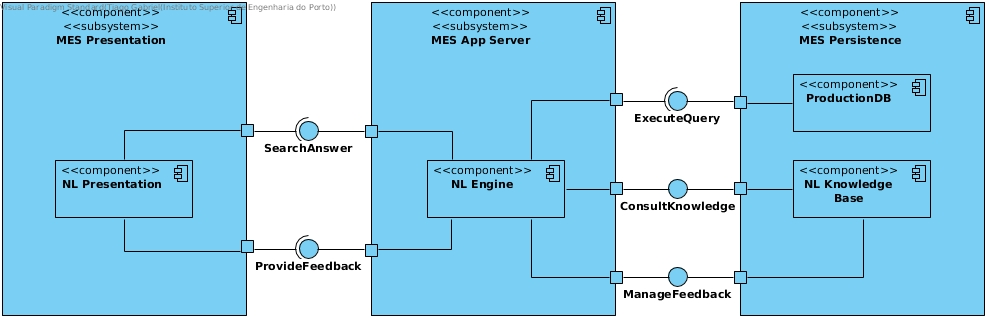
\includegraphics[width=\textwidth]{ch04/assets/generic-architecture.jpg}
         \caption{Arquitetura genérica do protótipo}
         \label{fig:generic_architecture}
     \end{subfigure}
     \bigbreak
     \bigbreak
     \begin{subfigure}{\textwidth}
         \centering
         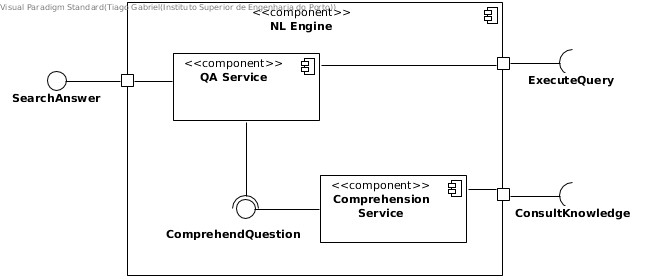
\includegraphics[width=.65\textwidth]{ch04/assets/nl-engine.jpg}
         \caption{Arquitetura detalhada do \textit{NL Engine}}
         \label{fig:nlengine_architecture}
     \end{subfigure}
\caption{Arquitetura do protótipo, apresentando um vista genérica e uma mais específica do componente \textit{NL Engine}}
\label{fig:model_architecture}
\end{figure}
%
\begin{itemize}
    \item 
    {
        \textit{NL Presentation} -- responsável pela interação com o utilizador. Integra a camada de apresentação do {\productname} e, como tal, é desenvolvido de acordo com as especificidades do subsistema em que se insere;
    }
    \item 
    {
        \textit{NL Engine} -- o módulo de linguagem natural, ou seja, o \inquotes{motor} que permite a tradução de linguagem natural em intenções e respetivas entidades. Integra a camada aplicacional de serviços do produto;
    }
    \item 
    {
        \textit{QA Service} -- trata-se de um subcomponente o \textit{NL Engine}, que conhece as partes envolvidas no processo de aquisição de resposta, sendo responsável por orquestrar esse processo. Trabalha em conjunto com o \textit{Comprehension Service} com o objetivo de identificar e mapear a intenção e entidades de uma dada \textit{query} de linguagem natural para obter a resposta da fonte de dados produtivos. Numa analogia à anatomia humana, pode ser considerado o \inquotes{cérebro} do processo;
    }
    \item 
    {
        \textit{Comprehension Service} -- outro subcomponente do \textit{NL Engine}, trabalha com a base de conhecimento definida (\textit{NL Knowledge Base}) para executar a tarefa de compreender a pergunta colocada. É neste componente que se insere a ferramenta escolhida para processamento de linguagem natural;
    }
    % \item 
    % {
    %     \textit{Feedback Management} -- tem a responsabilidade de gerir o \textit{feedback} providenciado pelo utilizador e disponibiliza serviços para a gestão dessa mesma informação, que incluem o desencadear do processo de aprendizagem, por exemplo. Inicialmente, o \textit{feedback} pode ser consultado manualmente, possibilitando o uso dessa informação para a melhoria do sistema. Contudo, podem ser aplicadas estratégias que façam uso desta informação de forma automática;
    % }
    \item 
    {
        \textit{NL Knowledge Base} -- base de conhecimento de domínio, incluída na camada de persistência do {\productname}. É configurada pela equipa de desenvolvimento e deve mapear as entidades de domínio e as intenções em que estão envolvidas;
    }
    \item 
    {
        \textit{Production Store} -- armazém de dados de negócio. Contém a informação que o utilizador deseja obter através de linguagem natural.
    }
\end{itemize}

Apesar da elucidação acerca da responsabilidade de cada componente no sistema, é importante detalhar a forma como estes interagem entre si, para atingir o objetivo. A Figura~\ref{fig:model_sequence_diagram} mostra como se desenrola a comunicação entre os diversos componentes, que se passa a descrever: o utilizador (\textit{User}) questiona o sistema através da interface gráfica (\textit{NL Presentation}). A questão é encaminhada para o \textit{QA Service} que se encarrega de \inquotes{pedir} ao \textit{Comprehension Service} para que lhe forneça a compreensão sob a forma de representação intermediária. Posto isto, o \textit{Comprehension Service} consulta a base de conhecimento (\textit{NL Knowledge Base}) para obter o conteúdo existente e, aplicando modelos de \gls{ml}, faz o reconhecimento das intenções e entidades presentes na questão. O \textit{QA Service} trata de converter a representação numa linguagem compatível com o \textit{Production Store} e executa a \textit{query} gerada. Aquando a aquisição dos dados, o \textit{QA Service} trata de \inquotes{documentá-los}, ou seja, colocar metadados que sejam importantes para processamento posterior. Por fim, a \textit{NL Presentation} processa o resultado para que este seja apresentado num formato adequado ao utilizador.

\begin{sidewaysfigure}
    \centering
    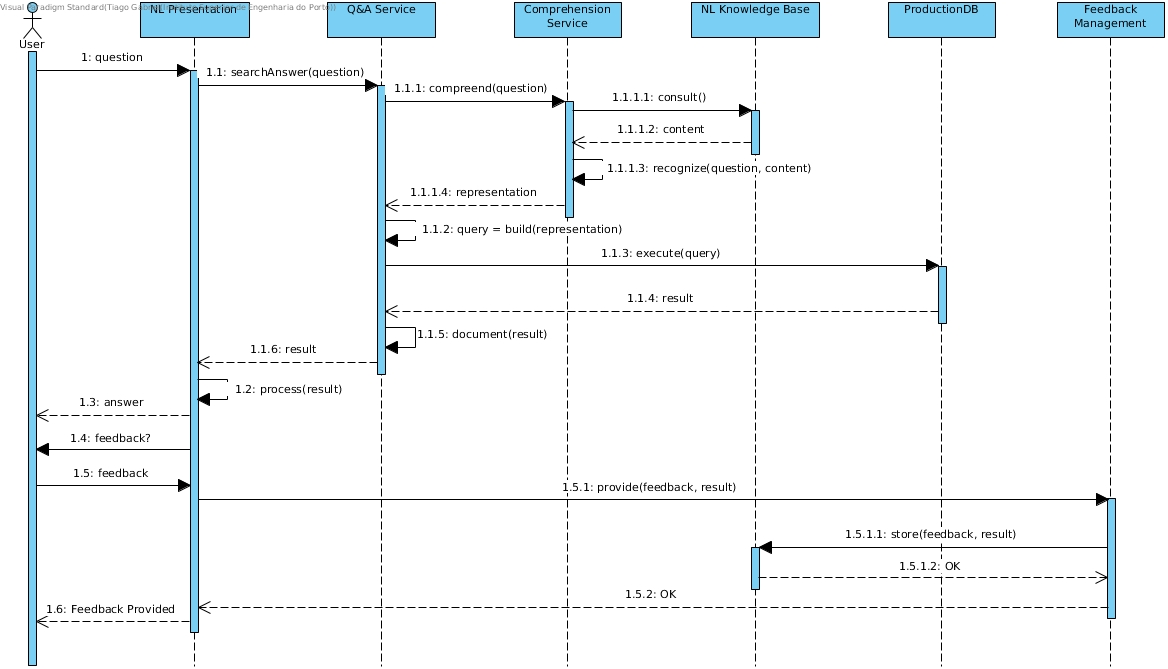
\includegraphics[width=\textwidth]{ch04/assets/workflow.jpg}
    \caption{Comunicação entre os componentes do módulo de linguagem natural}
    \label{fig:model_sequence_diagram}
\end{sidewaysfigure}

%%%%%%%%%%%%%%%%%%%%%%%%%%%%%%%%%
%           SECTION
%%%%%%%%%%%%%%%%%%%%%%%%%%%%%%%%%
\section{Síntese} 
\label{sec:chap04_chaptersummary}
Neste capítulo descreveu-se o processo que levou à especificação do módulo, dando ênfase aos detalhes da sua arquitetura. 

Começou-se por descrever a apreciação feita, em contexto prático, a algumas das ferramentas e abordagens anteriormente estudadas, fazendo referência aos seus pontos favoráveis e desfavoráveis. A conclusão retirada foi a de que a abordagem de reconhecimento de intenções e entidades seria a escolha adequada para o modelo a conceber.

Posteriormente, apresentou-se o modelo proposto, descrevendo a visão contemplada, as áreas funcionais -- \textit{QA} e \textit{Knowledge Base} -- e os casos de uso identificados, detalhando os mais importantes. Finalmente, a arquitetura num ponto de vista lógica, explicando os componentes e o fluxo de trabalho entre eles, no qual se apresenta um cenário genérico do funcionamento do processo de tradução e resposta.
